\documentclass[border=6pt]{standalone}
\usepackage{tikz}
\usetikzlibrary{arrows.meta,positioning,shapes.geometric,shapes.multipart,calc,fit,backgrounds,decorations.pathreplacing,decorations.markings,automata,chains,matrix,patterns}
\usepackage{circuitikz}
\usepackage{amsmath}
\usepackage{amssymb}
\begin{document}
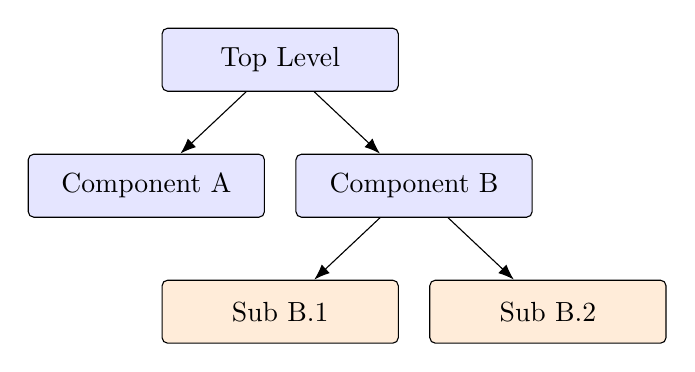
\begin{tikzpicture}[
  box/.style={rectangle, draw, fill=blue!10, rounded corners=2pt, minimum width=3cm, minimum height=0.8cm, align=center},
  level distance=1.6cm,
  level 1/.style={sibling distance=3.4cm},
  level 2/.style={sibling distance=3.4cm},
  edge from parent/.style={draw, -{Latex[length=2mm]}}
]
  \node[box] (root) {Top Level}
    child { node[box] (a) {Component A} }
    child { node[box] (b) {Component B}
      child { node[box, fill=orange!15] (b1) {Sub B.1} }
      child { node[box, fill=orange!15] (b2) {Sub B.2} }
    };
\end{tikzpicture}
\end{document}
